\documentclass[a4paper]{article}
\usepackage[12pt]{extsizes}
\usepackage{amsmath,amsthm,amssymb}
\usepackage[hidelinks]{hyperref} 
\usepackage[warn]{mathtext}
\usepackage[T1,T2A]{fontenc}
\usepackage[utf8]{inputenc}
\usepackage[english,russian]{babel}
\usepackage{tocloft}
\linespread{1.5}
\usepackage{indentfirst}
\usepackage{setspace}
%\полуторный интервал
\onehalfspacing

\newcommand{\RomanNumeralCaps}[1]
    {\MakeUppercase{\romannumeral #1}}

\usepackage{amssymb}

\usepackage{graphicx, float}
\graphicspath{{pictures/}}
\DeclareGraphicsExtensions{.pdf,.png,.jpg}
\usepackage[left=25mm,right=1cm,
    top=2cm,bottom=20mm,bindingoffset=0cm]{geometry}
\renewcommand{\cftsecleader}{\cftdotfill{\cftdotsep}}

\addto\captionsrussian{\renewcommand{\contentsname}{СОДЕРЖАНИЕ}}

\usepackage{fancyhdr}
\usepackage[nottoc]{tocbibind}

\fancypagestyle{plain}{
\fancyhf{}
\renewcommand{\headrulewidth}{0pt}
\fancyhead[R]{\thepage}
}

\usepackage{blindtext}
\pagestyle{myheadings}
\usepackage{hyperref}

\begin{document}
\begin{titlepage}
  \begin{center}
    \large
    Санкт-Петербургский политехнический университет Петра Великого
    
    Институт прикладной математики и механики
    
    \textbf{Высшая школа прикладной математики и вычислительной физики}
    \vfill
    \textsc{\textbf{\Large{Отчёт по лабораторной работе №1}}}\\[5mm]
    \\ по дисциплине\\ <<Математическая статистика>>\\
\end{center}

\vfill

\begin{tabular}{l p{140} l}
Выполнила студентка \\группы 5030102/90201 && Кожевникова Диана Геннадьевна \\
\\
Проверил\\Доцент, к.ф.-м.н.& \hspace{0pt} &   Баженов Александр Николаевич \\\\
\end{tabular}

\hfill \break
\hfill \break
\begin{center} Санкт-Петербург \\2022 \end{center}
\thispagestyle{empty}
\end{titlepage}
\newpage
\newpage
\begin{center}
    \setcounter{page}{2}
    \tableofcontents
\end{center}
\newpage
\begin{center}
    \setcounter{page}{3}
    \listoffigures
\end{center}
\newpage

\section {Постановка задачи}
\noindent Для 4 распределений:
\begin{itemize}
	\item Нормальное распределение $N(x, 0, 1)$ 
	\item Распределение Коши  $C(x, 0, 1)$
	\item Распределение Пуассона $P(k, 10)$
	\item Равномерное распределение $U(x, -\sqrt{3}, \sqrt{3})$
\end{itemize}
\begin{enumerate}
    \item Сгенерировать выборки размером 10, 100 и 1000 элементов.\newline Построить на одном рисунке гистограмму и график плотности распределения.
    \item Сгенерировать выборки размером 10, 100 и 1000 элементов.\newline Для каждой выборки вычислить следующие характеристики положения данных:\newline $\overline{x}, med x, z_R, z_Q, z_{tr}$. Повторить такие вычисления 1000 раз для каждой выборки и найти среднее характеристик положения и их квадратов:
        \begin{equation}
            E(z) = \overline{z}
        \end{equation}
        \newline Вычислить оценку дисперсий по формуле:
        \begin{equation}
            D(z) = \overline{z^2} - \overline{z}^2
        \end{equation}
        \newline Представить полученные данные в виде таблиц
    \item Сгенерировать выборки размером 20 и 100 элементов.
        \newline Построить для них боксплот Тьюки.
        Для каждого распределения определить долю выбросов экспериментально (сгенерировав выборку, соответствующую распределению 1000
        раз, и вычислив среднюю долю выбросов) и сравнить с результатами,
        полученными теоретически.
    \item Сгенерировать выборки размером 20, 60 и 100 элементов.\newline Построить на них эмпирические функции распределения и ядерные
    оценки плотности распределения на отрезке [−4; 4] для непрерывных распределений и на отрезке [6; 14] для распределения Пуассона.
\end{enumerate}


\section {Теория}

\subsection{Рассматриваемые распределения}
	\begin{itemize}
		\item Нормальное распределение \begin{equation}
										  N(x, 0, 1) = \frac{1}{\sqrt{2\pi}}e^{\frac{-x^2}{2}} \label{norm} 
									   \end{equation}
		\item Распределение Коши \begin{equation}
									C(x, 0, 1) = \frac{1}{\pi}\frac{1}{x^2+1} \label{koshi}
								 \end{equation} 
		\item Распределение Пуассона \begin{equation}
										P(k, 10) = \frac{10^k}{k!}e^{-10}\label{puasson}
									 \end{equation}
		\item Равномерное распределение \begin{equation}
				U(x, -\sqrt{3}, \sqrt{3}) =
				\begin{cases}
					\frac{1}{2\sqrt{3}} &\text{, |x|\leq \sqrt{3}$}\\
					0 &\text{, |x|>\sqrt{3}$}
				\end{cases}
				\label{uni} 
			\end{equation}
	\end{itemize}

	\subsection{Гистограмма}
	\subsubsection{Построение гистограммы}
	\noindent  Множество значений, которое может принимать элемент выборки, разбивается на несколько интервалов. Чаще всего эти интервалы берут одинаковыми, но это не является строгим требованием. Эти интервалы откладываются на горизонтальной оси, затем над каждым рисуется прямоугольник. Если все интервалы были одинаковыми, то высота каждого прямоугольника пропорциональна числу элементов выборки, попадающих в соответствующий интервал. Если интервалы разные, то высота прямоугольника выбирается таким образом, чтобы его площадь была пропорциональна числу элементов выборки, которые попали в этот интервал.
	
	\subsection{Вариационный ряд}
	\noindent Вариационным ряд - последовательность элементов выборки, расположенных в неубывающем порядке. Одинаковые элементы повторяются.
	
	\subsection{Выборочные числовые характеристики}
	\subsubsection{Характеристики положения}
	\begin{itemize}
	    \item Выборочное среднее
	    \begin{equation}
	        \overline{x} = \frac{1}{n}\sum_{i=1}^{n}{x_i}
	    \end{equation}
	    \item Выборочная медиана
	    \begin{equation}
	        med x = \begin{cases}
	            x_{(l+1)} &\text{, $ n=2l+1$}\\
				\frac{x_{(l)} + x_{(l+1)}}{2} &\text{, $ n=2l$}
	        \end{cases}
	    \end{equation}
	    \item Полусумма экстремальных выборочных элементов
	    \begin{equation}
	        z_R = \frac{x_{(1)} + x_{(n)}}{2}
	    \end{equation}
	    \item Полусумма квартилей
	    \newline Выборочная квартиль $z_p$ порядка $p$ определяется формулой:
	    \begin{equation}
	        z_p = \begin{cases}
	            x_{(|np|+1)} &\text{, $ np$ дробное}\\
				x_{(np)} &\text{, $ np$ целое}
	        \end{cases}
	    \end{equation}
	    \newline Полусумма квартилей
	    \begin{equation}
	       z_Q = \frac{z_{1/4} + z_{3/4}}{2}
	    \end{equation}
	    \begin{equation}
	        z_{tr} =\frac{1}{n-2r}\sum_{i=r+1}^{n-r}{x_{(i)}},
	        r\approx\frac{n}{4}
	    \end{equation}
	\end{itemize}
	\subsubsection{Характеристики рассеяния}
	\noindent Выборочная дисперсия
	\begin{equation}
		D = \frac{1}{n}\sum_{i=1}^{n}{(x_i-\overline{x})^2}
	\end{equation}
	\subsection{Боксплот Тьюки}
	\subsubsection{Построение}
	\noindent Границами ящика – первый и третий квартили, линия в середине ящика- медиана. Концы усов — края статистически значимой выборки (без выбросов). Длина «усов»:
	\begin{equation}
	    {X_1 = Q_1} - \frac{3}{2}{(Q_3 - Q_1)}, {X_2 = Q_3} + \frac{3}{2}{(Q_3 - Q_1)},
	\end{equation}
    где $X_1$ — нижняя граница уса, $X_$2— верхняя граница уса, $Q_1$— первый
    квартиль, $Q_2$ — третий квартиль.
    Данные, выходящие за границы усов (выбросы), отображаются на графике в виде маленьких кружков.

	\subsection{Теоретическая вероятность выбросов}
	\noindent Можно вычислить теоретические первый и третий квартили распределений $-Q_1^T$ и $-Q_3^T$.  По формуле (14) – теоретические нижнюю и верхнюю границы уса $-X_1^T$ и $-X_2^T$. Выбросы- величины $x$:
	    \begin{equation}
		    \left[
		    \begin{gathered}
		    x < X_1^T \\
		    x > X_2^T \\
		    \end{gathered}
		    \right.
	    \end{equation}
	Теоретическая вероятность выбросов:
	\begin{itemize}
	    \item для непрерывных распределений
	    \begin{equation}
		    P_B^T = P(x<X_1^T) + P(x>X_2^T)=F(X_1^T) + (1-F(X_2^T))
	    \end{equation}
	    \item для дискретных распределений
	    \begin{equation}
		    P_B^T = P(x<X_1^T)+P(x>x_2^T)=(F(X_1^T)-P(x=X_1^T))+(1-F(X_2^T))
	    \end{equation}
	\end{itemize}
	Выше $F(X) = P(x\leq{X})$- функция распределения
	\subsection{Эмпирическая функция распределения}
	\subsubsection{Статический ряд}
	\noindent Статистическим ряд- последовательность различных элементов выборки $z_1, z_2, ..., z_k$ положенных в возрастающем порядке с указанием частот $n_1, n_2, ..., n_k$, с которыми эти элементы содержатся в выборке. Обычно записывается в виде таблицы.
	\subsubsection{Эмпирическая функция распределения}
	\noindent Эмпирическая (выборочная) функция распределения (э.ф.р)- относительная частота события $X<x$, полученная по данной выборке:
	    \begin{equation}
            F_n^* = P^*(X<x)
        \end{equation}
	\subsubsection{ Нахождение эмпирической функции распределения}
	\noindent Для получения относительной частоты $P^*(X<x)$  просуммируем в статистическом ряде, построенном по данной выборке, все частоты $n_i$, для некоторых элементов $z_i$ статистического ряда меньше $x$. Тогда $P^*(X<x) = \frac{1}{n}\sum_{z_i<x}n_i$. Получаем
	\begin{equation}
        F^*(x)=\frac{1}{n}\sum_{z_i<x}n_i.
    \end{equation}
    $F^*(x)$-  функция распределения дискретной случайной величины $X^*$, заданной таблицей распределения
    \begin{table}[H]
    \centering
    \begin{tabular}{|c|c|c|c|c|}
        \hline
         $X^*$&$z_1$&$z_2$&...&$z_k$\\
         \hline
         $P$&$n_1/n$&$n_2/n$&...&$n_k/n$\\
         \hline
    \end{tabular}
    \caption{Таблица распределения}
    \label{tab:my_label}
    \end{table}
    Эмпирическая функция распределения является оценкой, т. е. приближённым значением, генеральной функции распределения
    \begin{equation}
        F_n^*(x)\approx F_X(x).
    \end{equation}
	\subsection{Оценки плотности вероятности}
	\subsubsection{Определение}
	\noindent Оценкой плотности вероятности $f(x)$ называется функция $\widehat{f}(x)$, построенная на основе выборки, приближённо равная $f(x)$
    \begin{equation}
        \widehat{f}(x)\approx f(x).
    \end{equation}
	\subsubsection{Ядерные оценки}
	\noindent Представим оценки в виде суммы с числом слагаемых, равным объёму выборки:\begin{equation}
        \widehat{f}_n(x)=\frac{1}{n h_n}\sum_{i=1}^n K\left(\frac{x-x_i}{h_n}\right).
    \end{equation}
    Здесь функция $K(u)$, называемая ядерной (ядром), непрерывна и является плотностью вероятности, $x_1,...,x_n$ $-$ элементы выборки, ${h_n}$ — любая последовательность положительных чисел, обладающая свойствами
    \begin{equation}
        h_n\xrightarrow[n\to\infty]{}0;\;\;\;\frac{h_n}{n^-1} \xrightarrow[n\to\infty]{}\infty.
    \end{equation}
    Такие оценки называются непрерывными ядерными [2, с. 421-423].\\\\
    Гауссово (нормальное) ядро
    \begin{equation}
        K(u)=\frac{1}{\sqrt{2\pi}}e^{-\frac{u^2}{2}}.
    \end{equation}
    Правило Сильвермана
    \begin{equation}
        h_n=\left(\frac{4\hat{\sigma}^5}{3n}\right)^{1/5}\approx1.06\hat{\sigma}n^{-1/5},
    \end{equation}
    где $\hat{\sigma}$ - выборочное стандартное отклонение.

\section {Реализация} 	
\noindent Лабораторная работа выполнена на языке Python версии 3.7 в среде разработки PyCharm. Использовались дополнительные библиотеки:
\begin{enumerate}
    \item scipy
    \item numpy
    \item matplotlib
    \item math
\end{enumerate}

\section {Результаты} 

\subsection{Гистограммы и графики плотности распределения}
	\begin{figure}[H]
		\centering
		\begin{tabular}{ccc}
			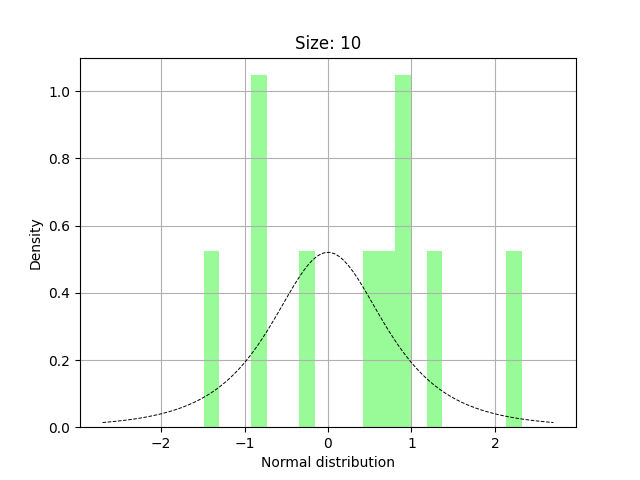
\includegraphics[width=55mm, height =0.15\textheight]{Figure_1.png}
			&
			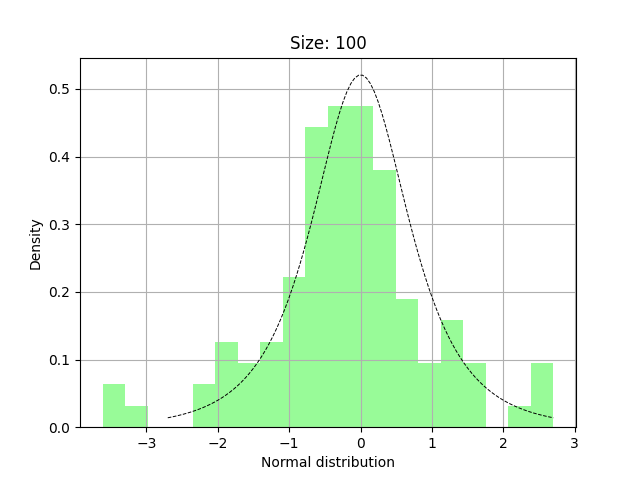
\includegraphics[width=55mm, height =0.15\textheight]{Figure_2.png}
			&
			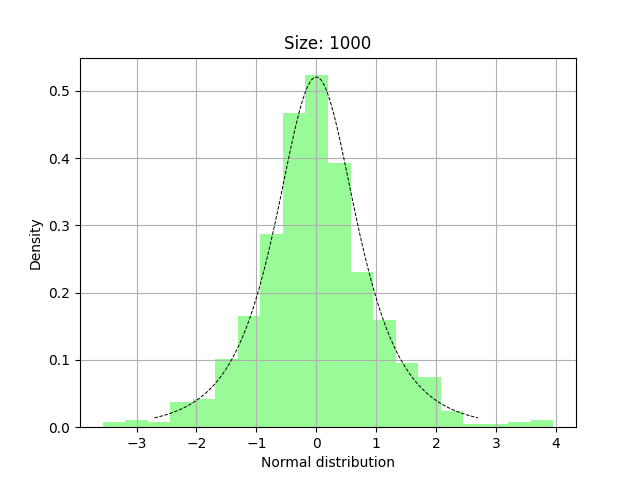
\includegraphics[width=55mm, height =0.15\textheight]{Figure_3.png}
		\end{tabular}
		\caption{Нормальное распределение} 
	\end{figure}

	\begin{figure}[H]
		\centering
		\begin{tabular}{ccc}
			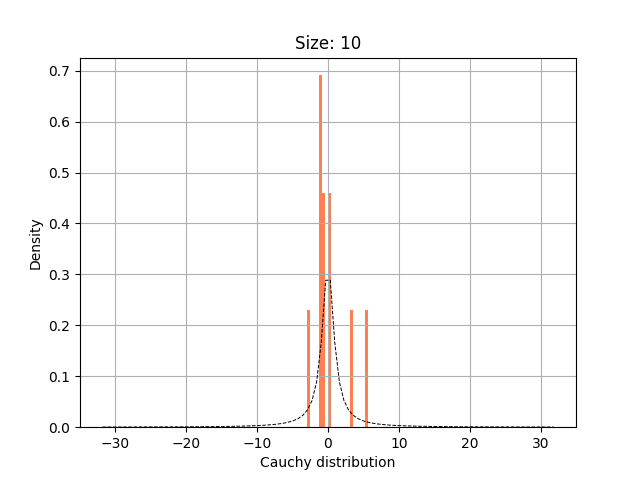
\includegraphics[width=55mm, height =0.15\textheight]{Figure_4.png}
			&
			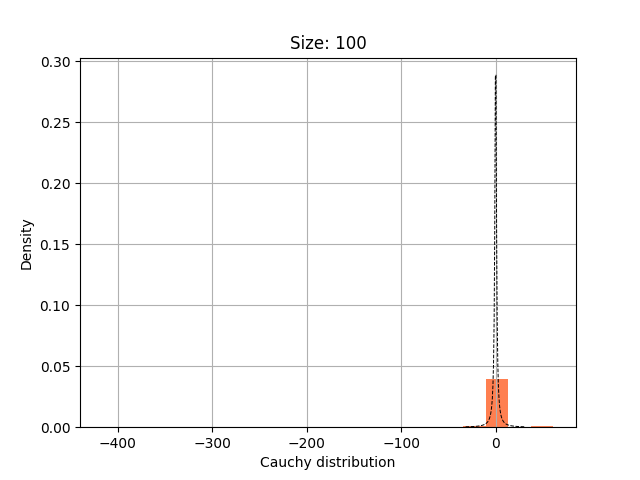
\includegraphics[width=55mm, height =0.15\textheight]{Figure_5.png}
			&
			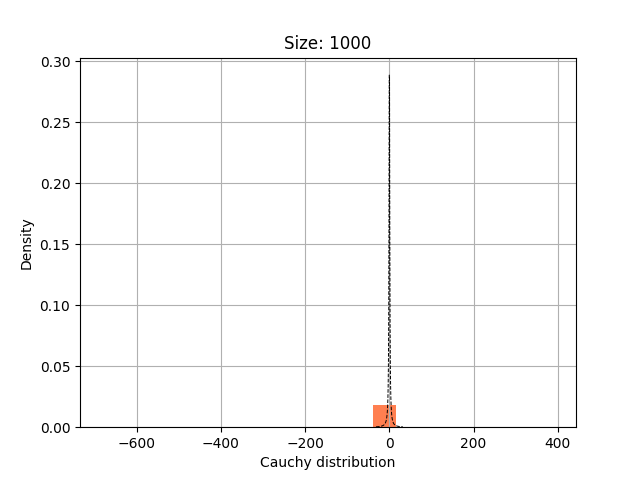
\includegraphics[width=55mm, height =0.15\textheight]{Figure_6.png}
		\end{tabular}
		\caption{Распределение Коши}
		\label{fig:cauchy}
	\end{figure}

	\begin{figure}[H]
		\centering
		\begin{tabular}{ccc}
			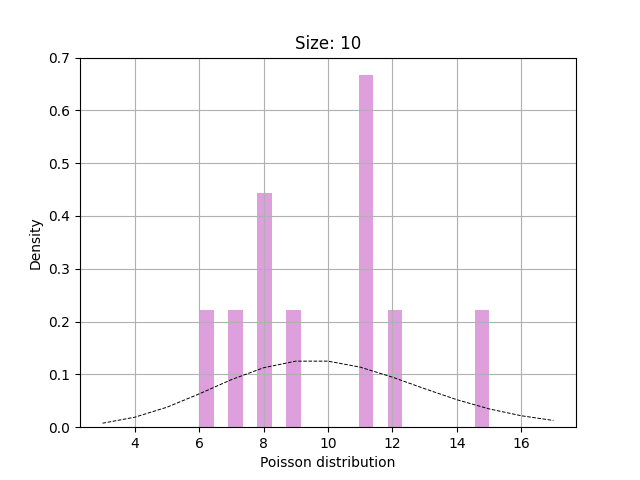
\includegraphics[width=55mm, height =0.15\textheight]{Figure_7.png}
			&
			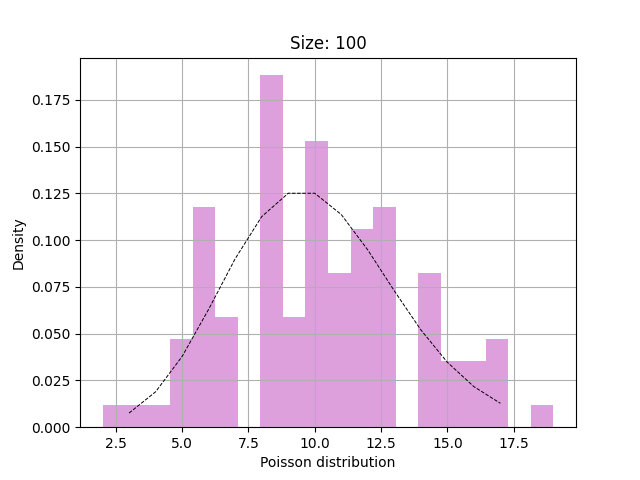
\includegraphics[width=55mm, height =0.15\textheight]{Figure_8.png}
			&
			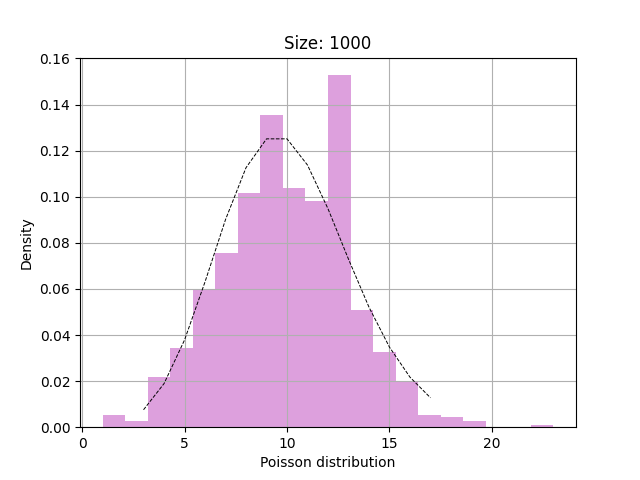
\includegraphics[width=55mm, height =0.15\textheight]{Figure_9.png}
		\end{tabular}
		\caption{Распределение Пуассона}
		\label{fig:poisson}
	\end{figure}

	\begin{figure}[H]
		\centering
		\begin{tabular}{ccc}
			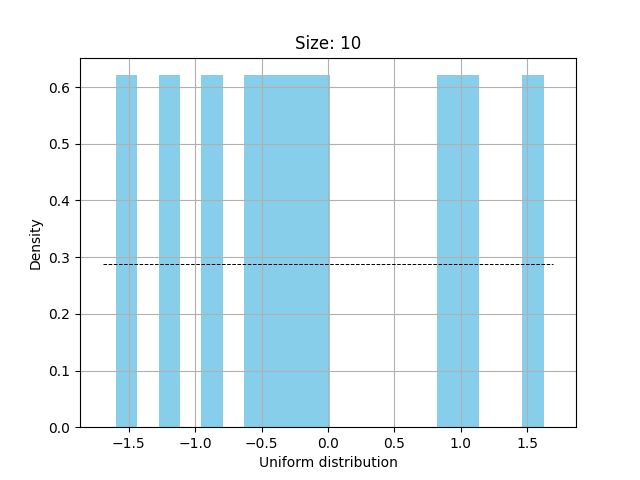
\includegraphics[width=55mm, height =0.15\textheight]{Figure_10.png}
			&
			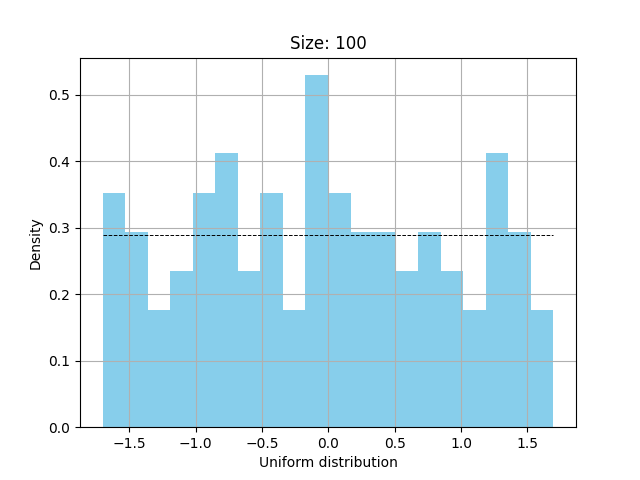
\includegraphics[width=55mm, height =0.15\textheight]{Figure_11.png}
			&
			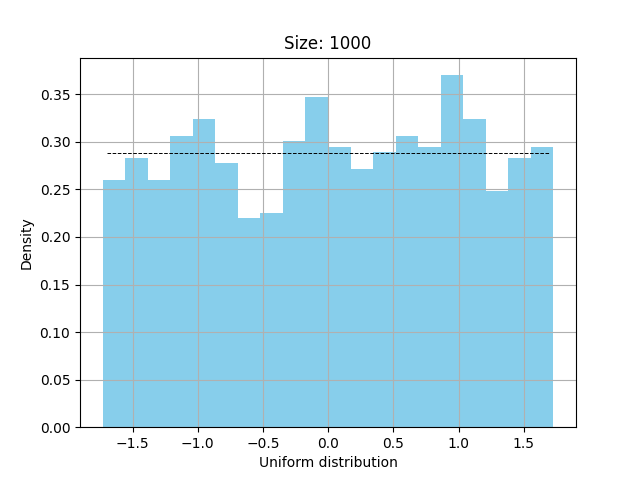
\includegraphics[width=55mm, height =0.15\textheight]{Figure_12.png}
		\end{tabular}
		\caption{Равномерное распределение}
		\label{fig:uniform}
	\end{figure}
\subsection{Характеристики положения и рассеяния}
\begin{table}[H]
		\centering
		\begin{tabular}[t]{|l|r|r|r|r|r|}
			\hline
			Characteristic   &      Mean &    Median &       $z_R$ &      $z_Q$ &      $z_{tr}$ \\
			\hline
			Normal E(z) 10   &  0.010232 & 0.018196 & 0.010349 & 0.32143 & 0.286511\\
			\hline
			Normal D(z) 10   &  0.095907 & 0.135498 & 0.183128 & 0.119274 & 0.1099\\
			\hline
			E(z) \pm \sqrt{D(z)} & [-0.299457; & [-0.349905; & [-0.417586; & [-0.02393; & [-0.0449999;\\
			& 0.319921] & 0.386297] & 0.438284] & 0.66679] & 0.618022]\\
			\hline
			\widehat{E}(z) & 0 & 0 & 0 & 0 & 0\\
			\hline
			Normal E(z) 100  & 0.003579 & 0.002227 & -0.013121 & 0.018929 & 0.029441\\
			\hline
			Normal D(z) 100  & 0.009892 & 0.014703 & 0.091264 & 0.012078 & 0.011253\\
			\hline
			E(z) \pm \sqrt{D(z)} & [-0.095877; & [-0.119029; & [-0.31522; & [-0.09097; & [-0.076639; \\
			&  0.103035] & 0.123483] & 0.288978] & 0.128828] & 0.135521] \\
			\hline
			\widehat{E}(z) & 0 & 0 & 0 & 0 & 0\\
			\hline
			Normal E(z) 1000 & 0.000983 & 0.000326 & -0.006743 & 0.00385 & 0.004204\\
			\hline
			Normal D(z) 1000 &  0.000933 & 0.001513 & 0.064184 & 0.001192 & 0.00116\\
			\hline
	    	E(z) \pm \sqrt{D(z)} & [-0.029558; & [-0.038566; & [-0.260088; & [-0.030672; & [-0.029852; \\
			&  0.031524] & 0.039218] & 0.246602] & 0.038372] & 0.03826] \\
			\hline
			\widehat{E}(z) & 0.0 & 0.0 & 0 & 0.0 & 0.0\\
			\hline
		\end{tabular}
		\caption{Нормальное распределение}
		\label{}
	\end{table}
	
	\begin{table}[H]
	\centering
		\begin{tabular}[t]{|l|r|r|r|r|r|}
			\hline
			Characteristic   &        Mean &    Median &            $z_R$ &       $z_Q$ &      $z_{tr}$ \\
			\hline
			Cauchy E(z) 10   &   0.653013 & -0.014515 & 3.409553 & 1.074588 & 0.657709\\
			\hline
			Cauchy D(z) 10   &  104.601594 & 0.34787 & 2451.630945, 3.7181 & 0.993591 \\
			\hline
			E(z) \pm \sqrt{D(z)} & [-9.574479; & [-0.60432; & [-46.104394; & [-0.853649; & [-0.339081; \\
		 	&  10.880505] & 0.575290] & 52.923500] & 3.002826] & 1.654499] \\
		 	\hline
			\widehat{E}(z) & - & 0 & - & - & -\\
			\hline
			Cauchy E(z) 100  &   5.618888 & -0.004478 & 282.391247 & 0.022293 & 0.034043 \\
			\hline
			Cauchy D(z) 100  & 17419.258926 & 0.023936 & 43556389.474686 & 0.052636 & 0.025721 \\
			\hline
		    E(z) \pm \sqrt{D(z)} & [-126.363152; & [-0.159191; & [-6317.335223; & [-0.207132; & [-0.126335; \\
			&  137.600928] & 0.150235] & 6882.117717] & 0.251718] & 0.194421] \\
			\hline
			\widehat{E}(z) & - & 0 & - & 0 & 0\\
			\hline
			Cauchy E(z) 1000 &   1.054504 & -0.000892 & 522.577434 & 0.000884 & 0.002404 \\
			\hline
			Cauchy D(z) 1000 & 2527.229116 & 0.002599 & 628236126.30319 & 0.004797 & 0.002624 \\
			\hline
			E(z) \pm \sqrt{D(z)} & [-49.21705; & [-0.051875; & [-24542.061528; & [-0.068379; & [-0.048823; \\
			&  51.326058] & 0.050091] & 25587.216396] & 0.070147] & 0.053631] \\
			\hline
			\widehat{E}(z) & - & 0.0 & - & 0.0 & 0.0\\
			\hline
		\end{tabular}
	\caption{Распределение Коши}
	\label{tab:cauchy}
	\end{table}

\begin{table}[H]
		\centering
		\begin{tabular}[t]{|l|r|r|r|r|r|}
			\hline
			Characteristic    &      Mean &   Median &       $z_R$ &      $z_Q$ &     $z_{tr}$ \\
			\hline
			Poisson E(z) 10   & 10.077 & 9.9545 & 10.401 & 10.9955 & 10.835667     \\
			\hline
			Poisson D(z) 10   & 1.043651 & 1.49268 & 1.973199 & 1.42673 & 1.312717  \\
			\hline
			E(z) \pm \sqrt{D(z)} & [9.055408; & [8.732747; & [8.99629; & [9.801042; & [9.689928; \\
			&  11.098592] & 11.176253] & 11.805706] & 12.189958] & 11.981406] \\
			\hline
			\widehat{E}(z) & 10^{+1}_{-1} & 10^{+1}_{-1} & 10^{+1}_{-1} & 11^{+1}_{-1} & 11^{+1}_{-1}\\
			\hline
			Poisson E(z) 100  & 9.98639 & 9.8205 & 10.959 & 9.954 & 9.92078 \\
			\hline
			Poisson D(z) 100  &  0.09173 & 0.19353 & 1.009319 & 0.143384 & 0.108617 \\
			\hline
			E(z) \pm \sqrt{D(z)} & [9.683521; & [9.380580; & [9.954351; & [9.575339; & [9.59121 \\
			&  10.289259] & 10.26042] & 11.963649] & 10.332661] & 10.250350] \\
			\hline
			\widehat{E}(z)  & 10^{+1}_{-1} & 10^{+1}_{-1} & 11^{+1}_{-1} & 10 & 10\\
			\hline
			Poisson E(z) 1000 & 9.997453 & 9.999 & 11.6285 & 9.995 & 9.865078 \\
			\hline
			Poisson D(z) 1000 &  0.0092 & 0.000999 & 0.689738 & 0.002475 & 0.010254 \\
			\hline
			E(z) \pm \sqrt{D(z)} & [9.901535; & [9.967393; & [10.797995; & [9.945251; & [9.763817; \\
			&  10.093371] & 10.030607] & 12.459005] & 10.044749 & 9.966339] \\
			\hline
			\widehat{E}(z) & 10^{+1}_{-1} & 10^{+1}_{-1} & 11^{+1}_{-1} & 10^{+1}_{-1} & 9^{+0.1}_{-0.1}\\
			\hline
		\end{tabular}
		
		\caption{Распределение Пуассона}
		\label{tab:poisson}
	\end{table}

\begin{table}[H]
		\centering
		\begin{tabular}[t]{|l|r|r|r|r|r|}
			\hline
			Characteristic    &      Mean &    Median &       $z_{R}$ &       $z_Q$ &      $z_{tr}$ \\
			\hline
			Uniform E(z) 10   &   -0.015273 & -0.019191 & -0.003179 & 0.30327 & 0.29953 \\
			\hline
			Uniform D(z) 10   &  0.094209 & 0.214514 & 0.043017 & 0.117182 & 0.144624 \\
			\hline
			E(z) \pm \sqrt{D(z)} & [-0.322209; & [-0.482348; & [-0.210584; & [-0.039049; & [-0.080765; \\
			&  0.291663] & 0.443966] & 0.204226] & 0.645589] & 0.679825] \\
			\hline
			\widehat{E}(z)  & 0 & 0 & 0 & 0 & 0\\
			\hline
			Uniform E(z) 100  & 0.003447 & 0.002554 & -0.001096 & 0.022267 & 0.03982 \\
			\hline
			Uniform D(z) 100  &  0.009041 & 0.0266 & 0.000546 & 0.013745 & 0.017917 \\
			\hline
			E(z) \pm \sqrt{D(z)} & [-0.091637; & [-0.160542; & [-0.024465; & [-0.094971; & [-0.094035; \\
			& 0.098531] & 0.16565] & 0.022273] & 0.139505] & 0.173675] \\
			\hline
			\widehat{E}(z) & 0.0 & 0 & 0.0 & 0 & 0\\
			\hline
			Uniform E(z) 1000 & -0.0001 & 0.000955 & 7.1e-05 & 0.000932 & 0.003488  \\
			\hline
			Uniform D(z) 1000 & 0.001001 & 0.003098 & 6e-06 & 0.001452 & 0.002022 \\
			\hline
			E(z) \pm \sqrt{D(z)} & [-0.031741; & [-0.054708; & [-0.00238; & [-0.037179; & [-0.041474; \\
			&  0.031541] & 0.056618] & 0.002522] & 0.039043] & 0.04845] \\
			\hline
			\widehat{E}(z)  & 0.0 & 0.0 & 0.00 & 0.0 & 0.0\\
			\hline
		\end{tabular}
		\caption{Равномерное распределение}
		\label{tab:uniform}
	\end{table}

	
\subsection{Боксплот Тьюки}
    \begin{figure}[H]
		\centering
		\begin{tabular}{ccc}
			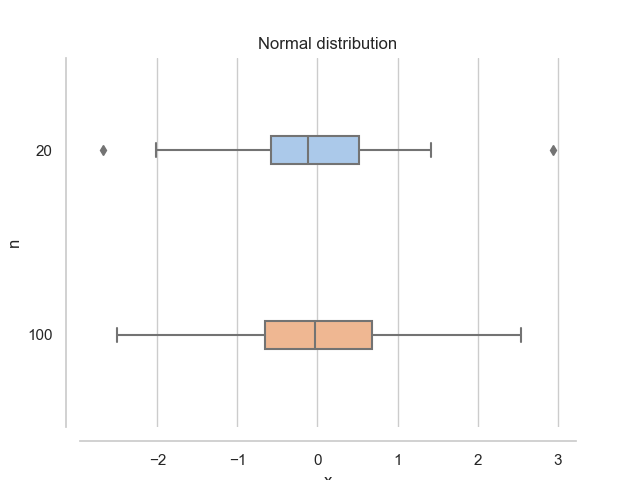
\includegraphics[width=90mm, height =0.25\textheight]{Box_1.png}
		\end{tabular}
		\caption{Нормальное распределение} 
	\end{figure}
	\begin{figure}[H]
		\centering
		\begin{tabular}{ccc}
			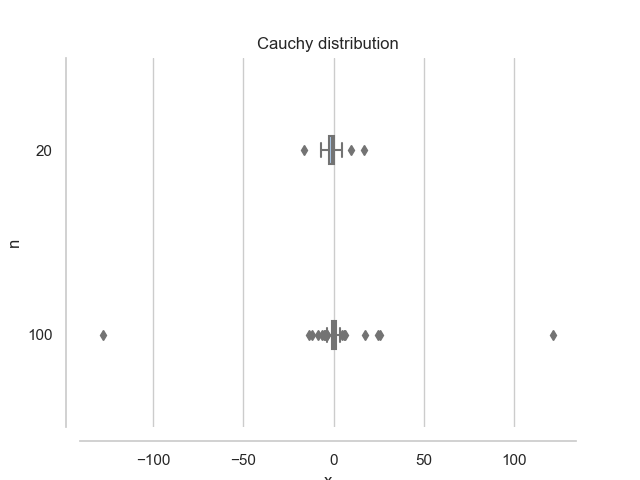
\includegraphics[width=90mm, height =0.25\textheight]{Box_2.png}
		\end{tabular}
		\caption{Распределение Коши} 
	\end{figure}
	\begin{figure}[H]
		\centering
		\begin{tabular}{ccc}
			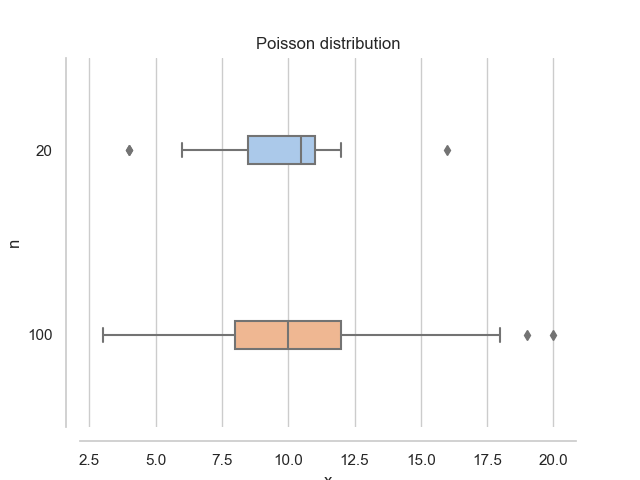
\includegraphics[width=90mm, height =0.25\textheight]{Box_3.png}
		\end{tabular}
		\caption{Распределение Пуассона} 
	\end{figure}
	\begin{figure}[H]
		\centering
		\begin{tabular}{ccc}
			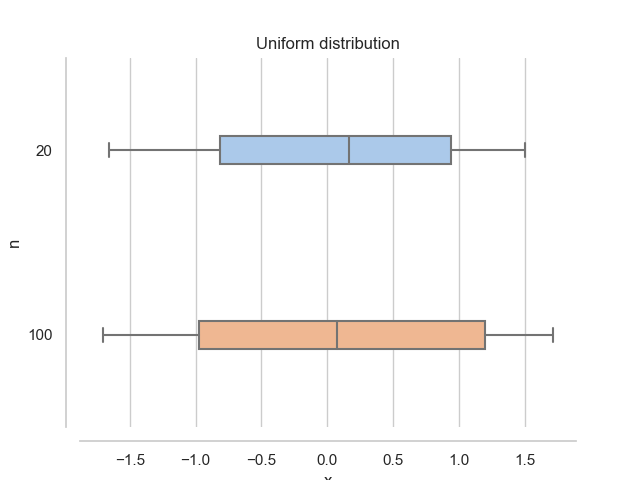
\includegraphics[width=90mm, height =0.25\textheight]{Box_4.png}
		\end{tabular}
		\caption{Равномерное распределение} 
	\end{figure}
\subsection{Доля выбросов}
\noindent Округление доли выбросов:\\
Выборка случайна, поэтому в качестве оценки рассеяния можно взять дисперсию пуассоновского потока:  $D_n \approx \sqrt{n}$\\
Доля $p_n = \frac{D_n}{n}=\frac{1}{\sqrt{n}}$\\
Доля $n=20: p_n=\frac{1}{\sqrt{20}}$ - примерно 0.2 или 20\% \\
Для $n=100: p_n=\frac{1}{\sqrt{100}}$ - примерно 0.1 или 10\% \\
Исходя из этого можно решить, сколько знаков оставлять в доле выброса.
\begin{table}[H]
		\centering
		\begin{tabular}[t]{lrr}
			\hline
			Выборка   &      Доля выбросов	& $P_B^T$		\\
			\hline
			Normal n=20   	&	0.02265 	& 0.007\\
			Normal n=100   	&  	0.01515		& 0.007\\
			Cauchy n=20 	& 	0.1521  	& 0.156\\
			Cauchy n=100	&  	0.1848 		& 0.156\\
			Poisson n=20	&	0.02615 	& 0.008\\
			Poisson n=100	&	0.01656		& 0.008\\
			Uniform n=20	&	0.00245 	& 0 	\\
			Uniform n=100	&	0.00049 	& 0	    \\
			\hline
		\end{tabular}
		\caption{Доля выбросов}
		\label{tab:normal}
	\end{table}


\subsection{Теоретическая вероятность выбросов}
\begin{table}[H]
		\centering
		\begin{tabular}[t]{lrrrrr}
			\hline
			Распределение   &      $Q_1^T$	& $Q_3^T$ & $X_1^T$ & $X_2^T$ & $P_B^T$	\\
			\hline
			Нормальное распределение 	& -0.674& 0.674 & -2.698 	&  2.698 	& 0.007 \\
			Распределение Коши 			& -1	& 1		&  -4		& 4			& 0.156 \\
			Распределение Пуассона 		& 8		& 12	& 2			& 18		& 0.008 \\
			Равномерное распределение 	&-0.866 & 0.866	& -3.464 	& 3.464 	& 0	\\
			
			\hline
		\end{tabular}
		\caption{Теоретическая вероятность выбросов}
		\label{tab:normal}
	\end{table}
\subsection{Эмпирическая функция распределения}
\begin{figure}[H]
	\centering
	{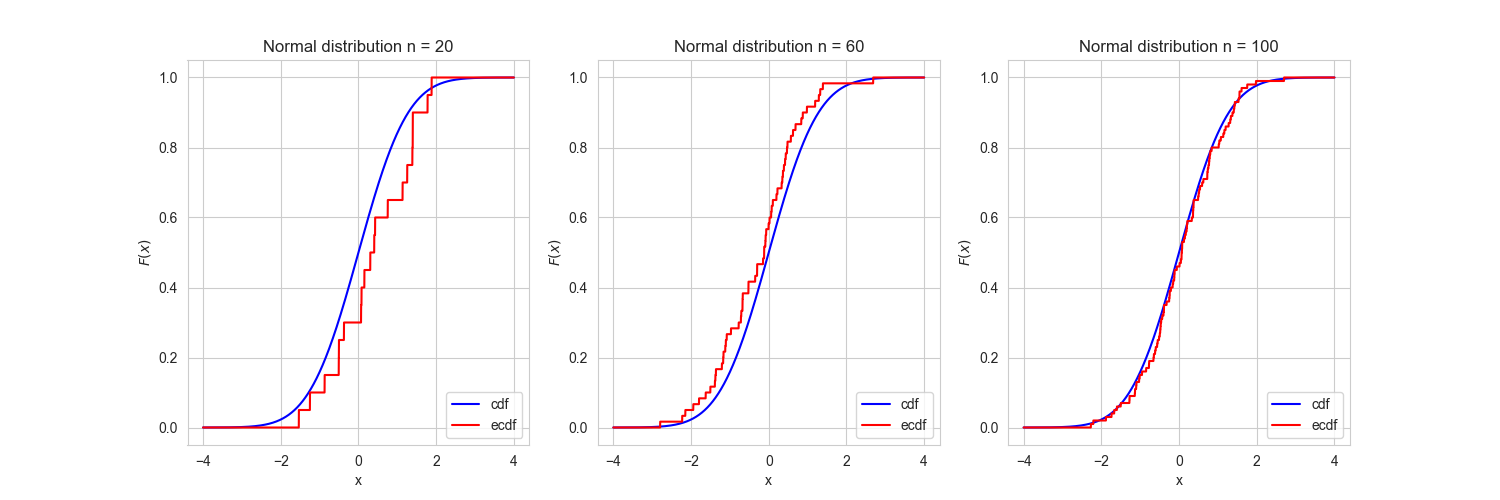
\includegraphics[scale=0.51]{Normal distribution100.png}}
		\caption{Нормальное распределение} 
		\label{fig:normal}
\end{figure}

\begin{figure}[H]
	{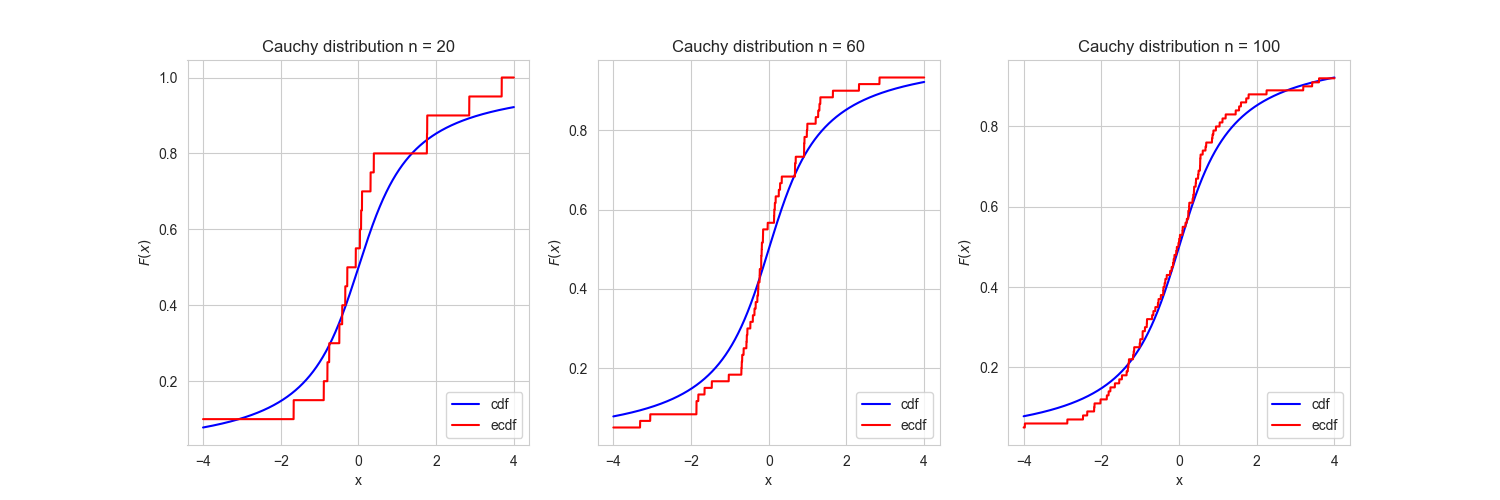
\includegraphics[scale=0.51]{Cauchy distribution100.png}}
		\caption{Распределение Коши} 
		\label{fig:normal}
	\end{figure}

\begin{figure}[H]
	{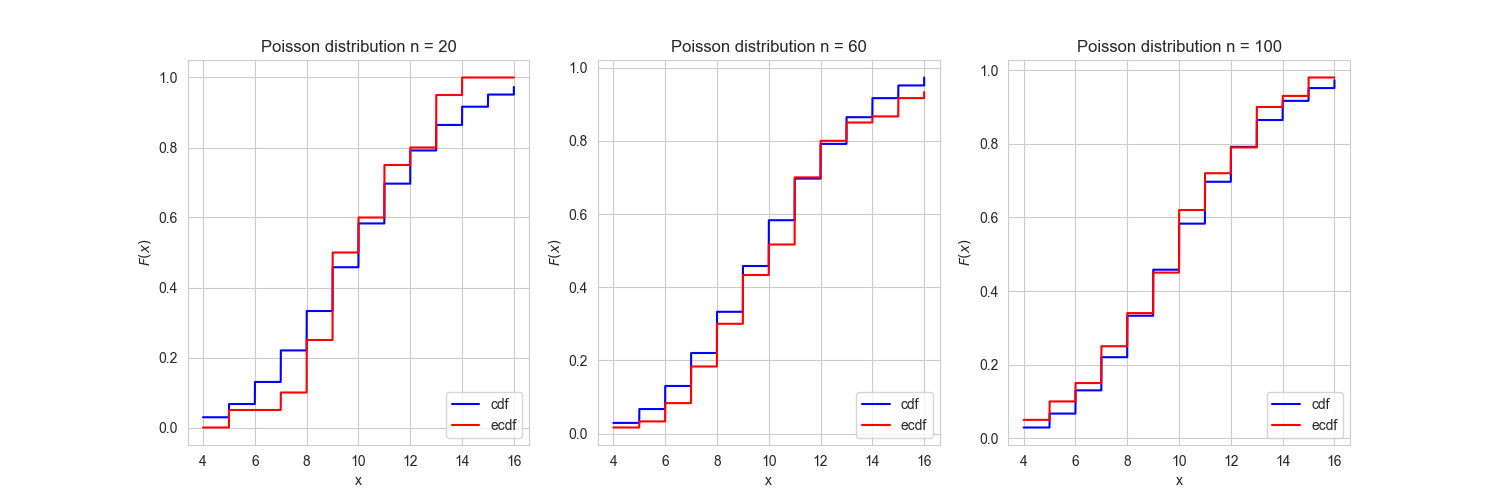
\includegraphics[scale=0.51]{Poisson distribution100.png}}
		\caption{Распределение Пуассона} 
		\label{fig:normal}
	\end{figure}
	
\begin{figure}[H]
	{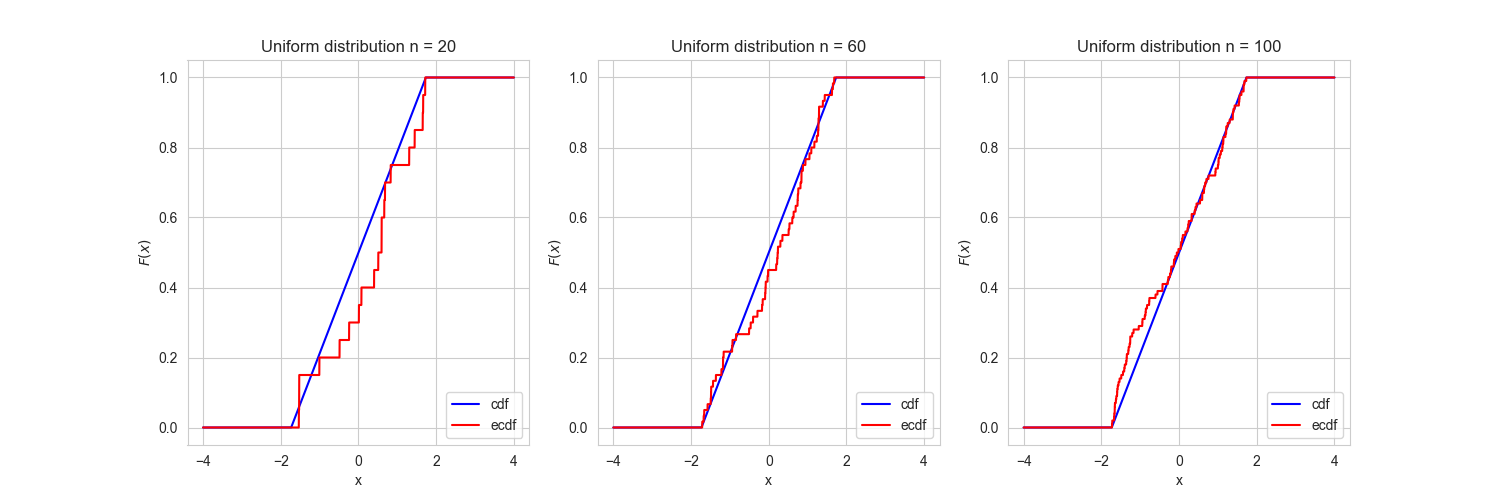
\includegraphics[scale=0.51]{Uniform distribution100.png}}
		\caption{Равномерное распределение} 
		\label{fig:normal}
	\end{figure}
	
\subsection{Ядерные оценки плотности распределения}
\begin{figure}[H]
	{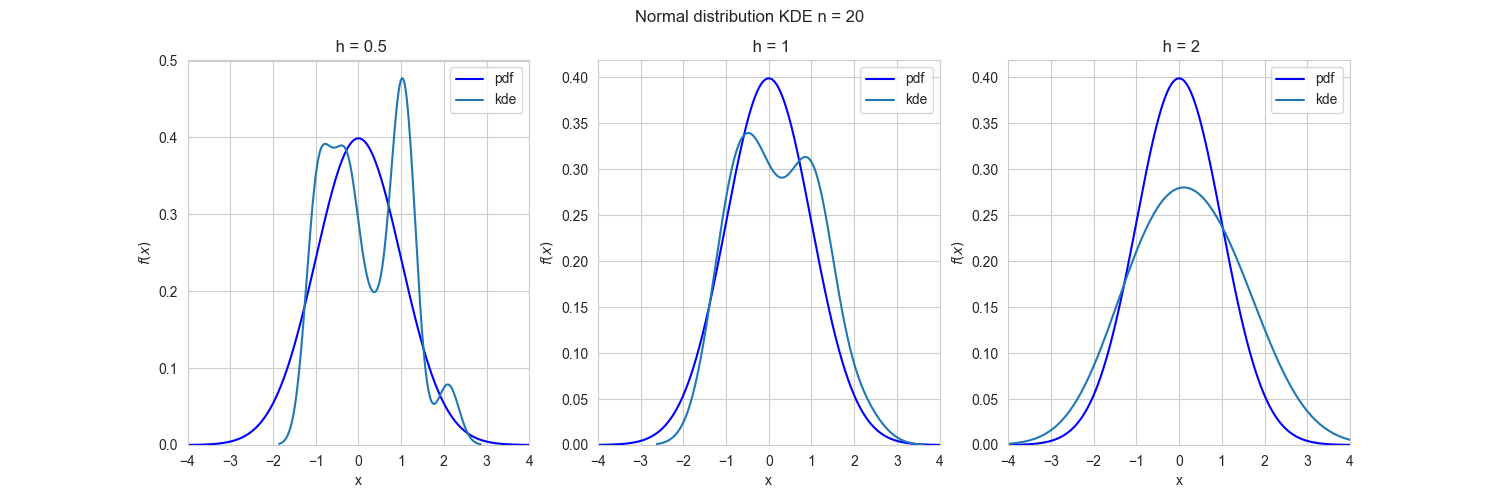
\includegraphics[scale=0.51]{Normal distributionKDE20.png}}
		\caption{Нормальное распределение, $n=20$} 
		\label{fig:normal}
	\end{figure}
	
\begin{figure}[H]
	{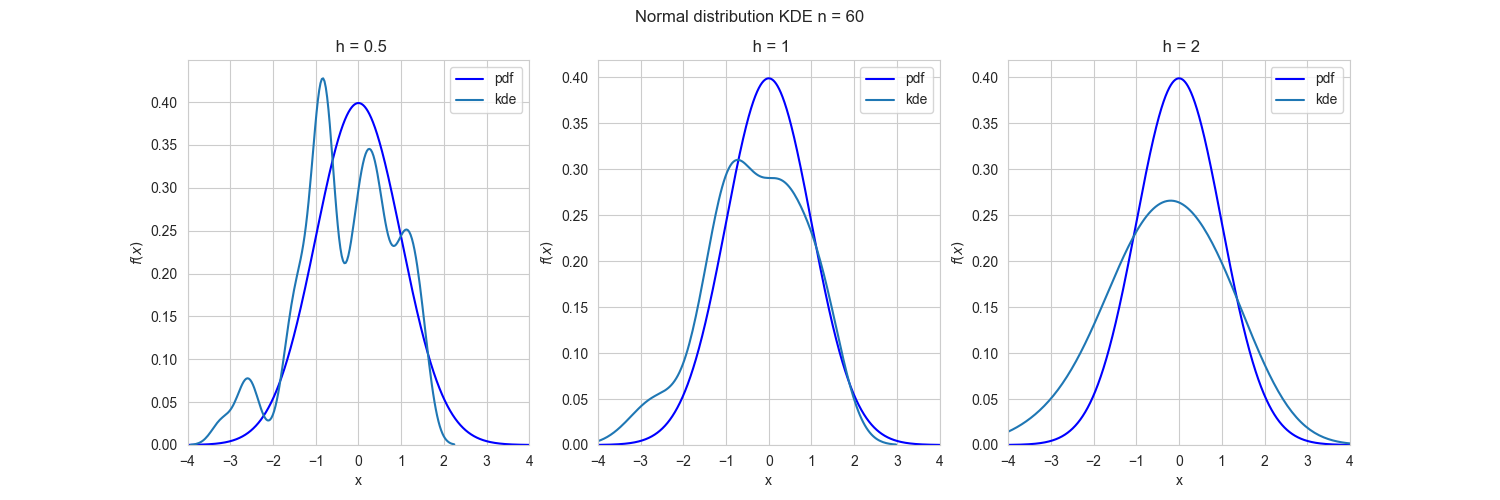
\includegraphics[scale=0.51]{Normal distributionKDE60.png}}
		\caption{Нормальное распределение, $n=60$} 
		\label{fig:normal}
	\end{figure}
		
\begin{figure}[H]
	{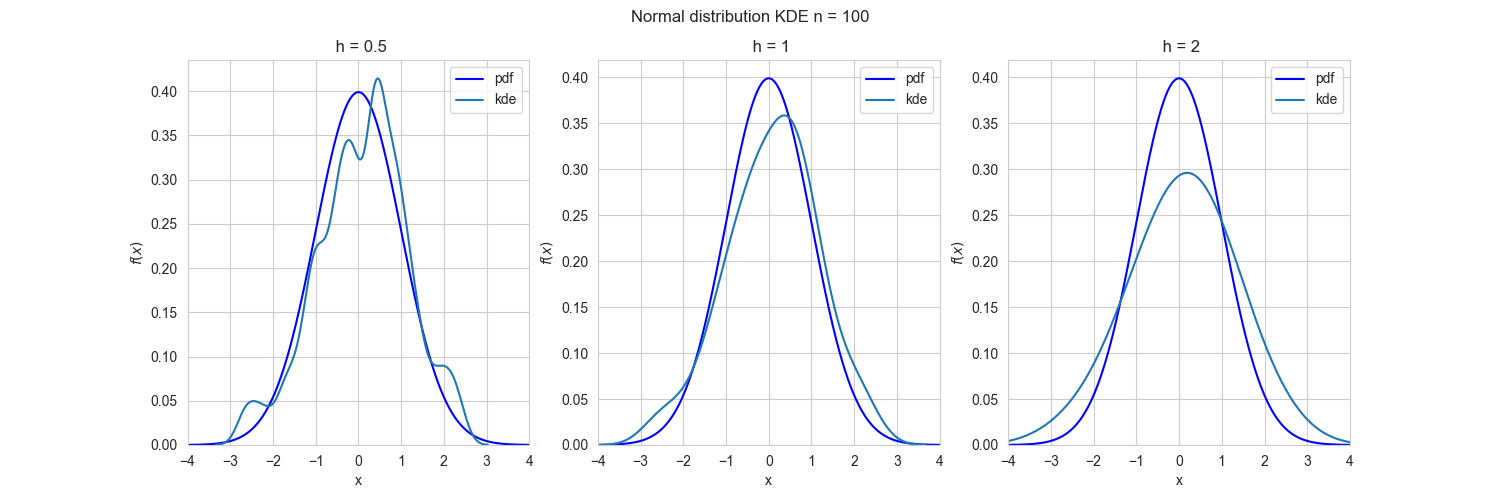
\includegraphics[scale=0.51]{Normal distributionKDE100.png}}
		\caption{Нормальное распределение, $n=100$} 
		\label{fig:normal}
	\end{figure}

\begin{figure}[H]
	{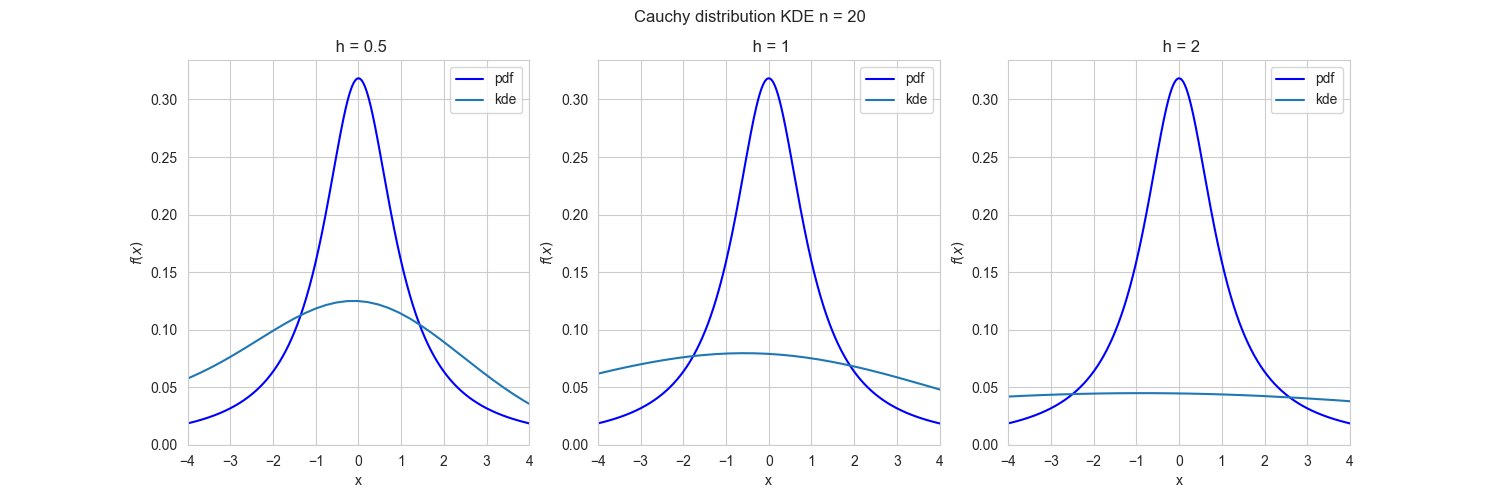
\includegraphics[scale=0.51]{Cauchy distributionKDE20.png}}
		\caption{Распределение Коши, $n=20$} 
		\label{fig:normal}
	\end{figure}
	
\begin{figure}[H]
	{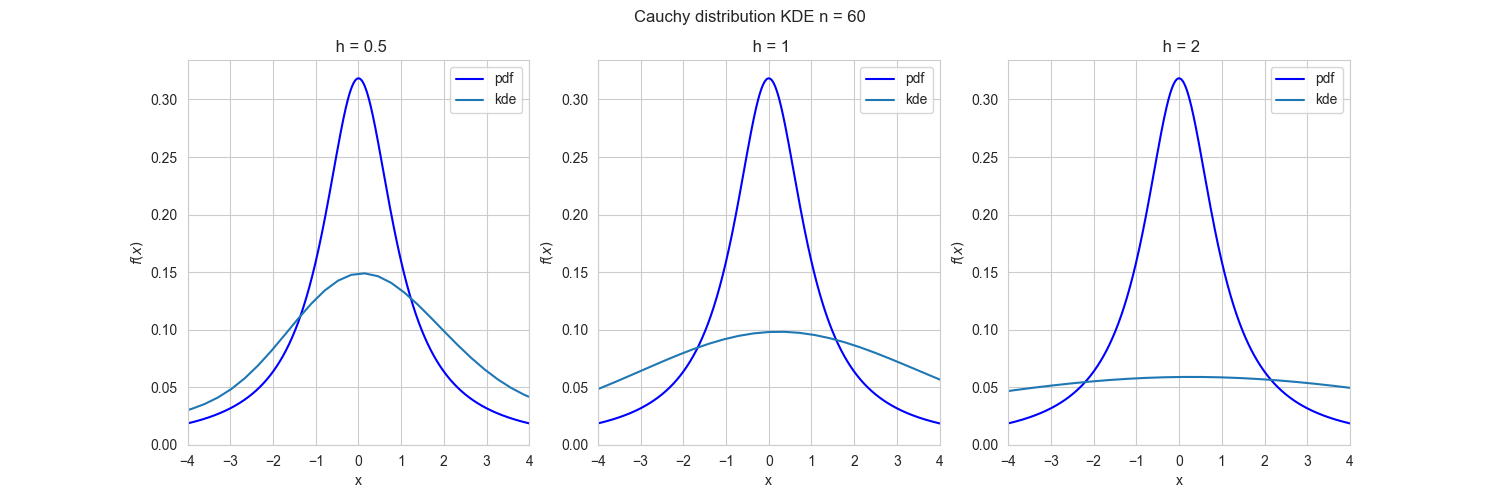
\includegraphics[scale=0.51]{Cauchy distributionKDE60.png}}
		\caption{Распределение Коши, $n=60$} 
		\label{fig:normal}
	\end{figure}
	
\begin{figure}[H]
	{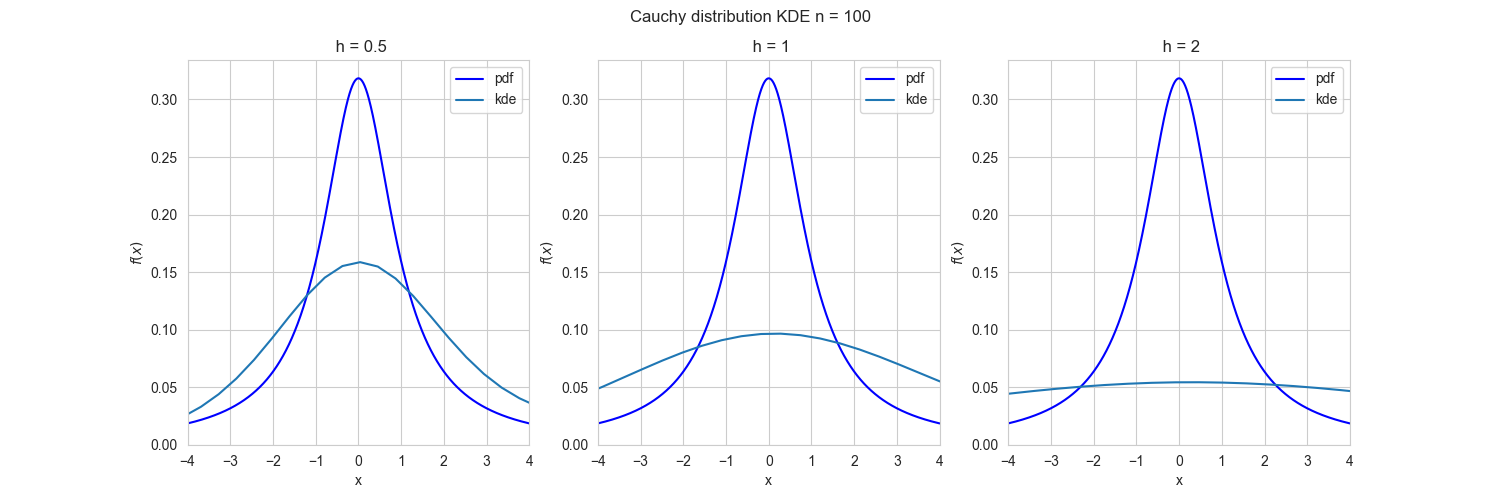
\includegraphics[scale=0.51]{Cauchy distributionKDE100.png}}
		\caption{Распределение Коши, $n=100$} 
		\label{fig:normal}
	\end{figure}

\begin{figure}[H]
	{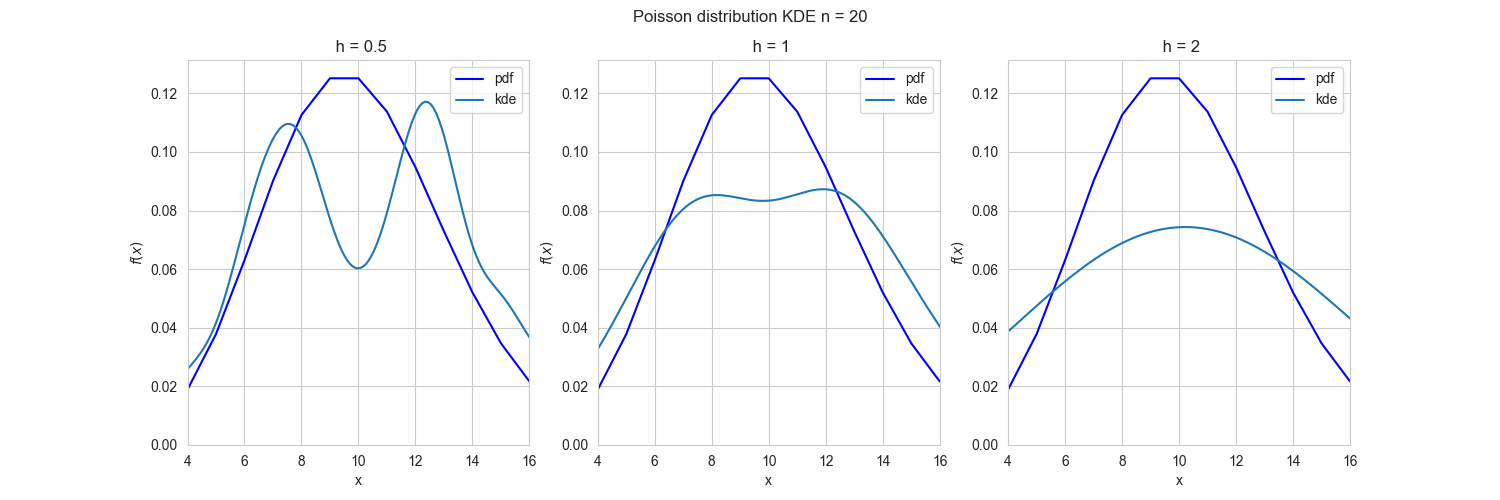
\includegraphics[scale=0.51]{Poisson distributionKDE20.png}}
		\caption{Распределение Пуассона, $n=20$} 
		\label{fig:normal}
	\end{figure}
	
\begin{figure}[H]
	{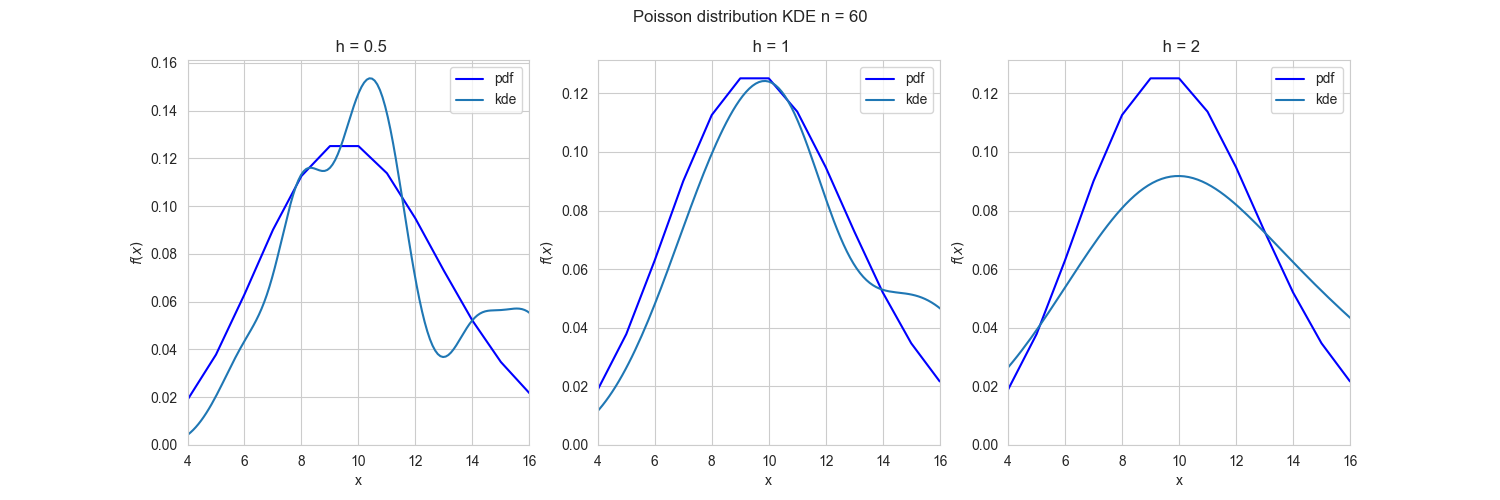
\includegraphics[scale=0.51]{Poisson distributionKDE60.png}}
		\caption{Распределение Пуассона, $n=60$} 
		\label{fig:normal}
	\end{figure}
	
\begin{figure}[H]
	{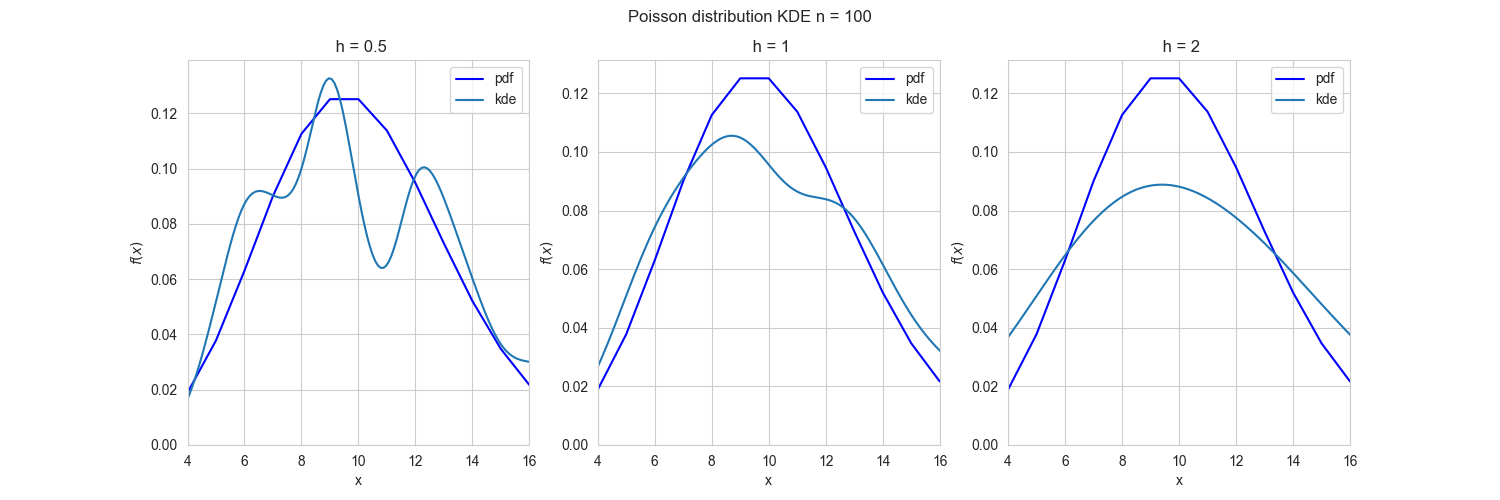
\includegraphics[scale=0.51]{Poisson distributionKDE100.png}}
		\caption{Распределение Пуассона, $n=100$} 
		\label{fig:normal}
	\end{figure}
	
\begin{figure}[H]
	{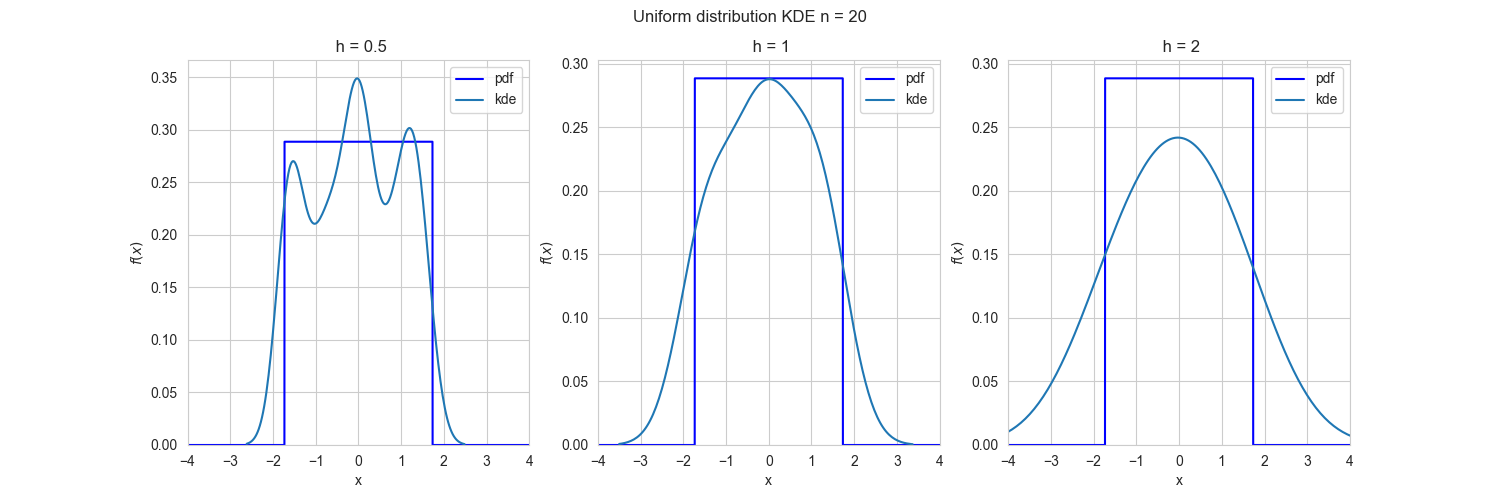
\includegraphics[scale=0.51]{Uniform distributionKDE20.png}}
		\caption{Равномерное распределение, $n=20$} 
		\label{fig:normal}
	\end{figure}
	
\begin{figure}[H]
	{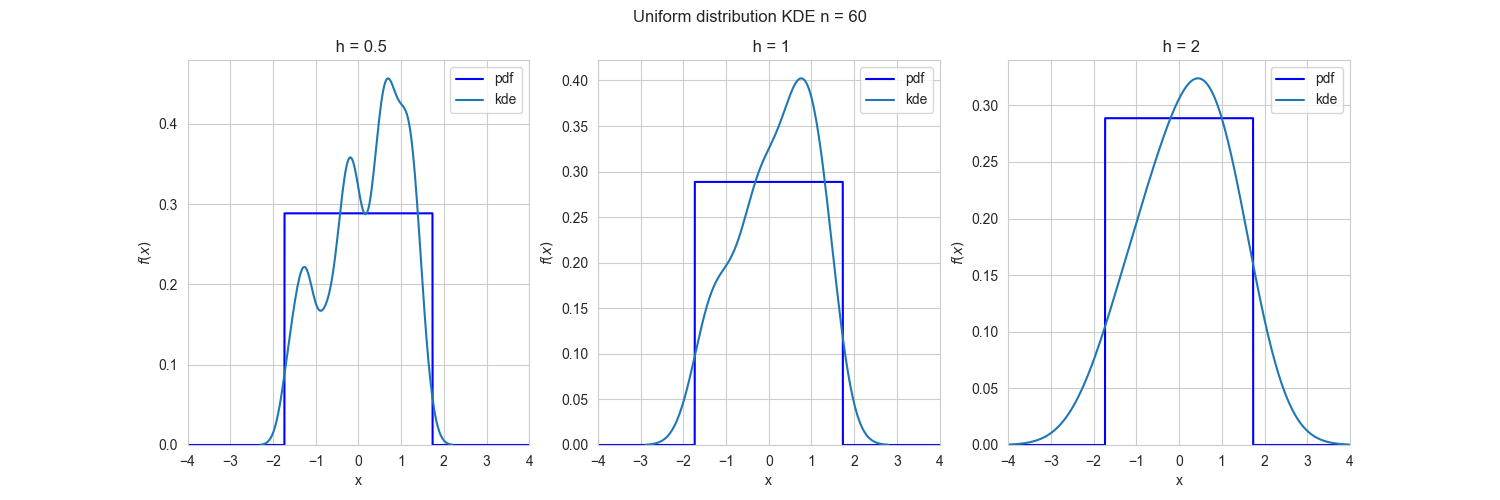
\includegraphics[scale=0.51]{Uniform distributionKDE60.png}}
		\caption{Равномерное распределение, $n=60$} 
		\label{fig:normal}
	\end{figure}

\begin{figure}[H]
	{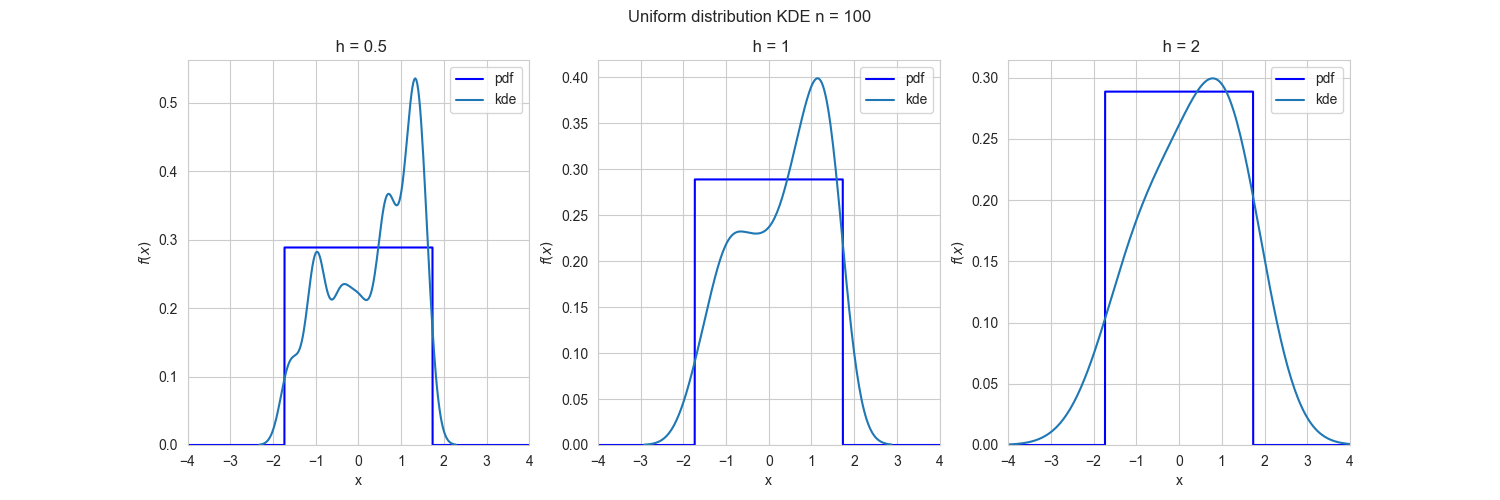
\includegraphics[scale=0.51]{Uniform distributionKDE100.png}}
		\caption{Равномерное распределение, $n=100$} 
		\label{fig:normal}
	\end{figure}
	
\section{Обсуждение}
\subsection{Гистограммы}
\noindent По результатам проделанной работы можем сделать вывод о том, что чем больше выборка для каждого из распределений, тем ближе ее гистограмма к графику плотности вероятности того закона, по которому распределены величины сгенерированной выборки. Чем меньше выборка, тем менее она показательна - тем хуже по ней определяется характер распределения величины. \newline Также можно заметить, что максимумы гистограмм и плотностей распределения почти нигде не совпали. Также наблюдаются всплески гистограмм,
что наиболее хорошо прослеживается на распределении Коши.
\subsection{Характеристики положения и рассеяния}
\noindent Исходя из данных, приведенных в таблицах, можно судить о том, что дисперсия характеристик рассеяния для распределения Коши является некой аномалией: значения слишком большие даже при увеличении размера выборки - понятно, что это результат выбросов, которые мы могли наблюдать в результатах предыдущего задания.
\subsection{Доля и теоретическая вероятность выбросов}
\noindent По данным, приведенным в таблице, можно сказать, что чем больше выборка, тем ближе доля выбросов будет к теоретической оценке. Снова доля
выбросов для распределения Коши значительно выше, чем для остальных распределений. Равномерное распределение же в точности повторяет теоретическую оценку - выбросов мы не получали. \newline Боксплоты Тьюки действительно позволяют более наглядно и с меньшими усилиями оценивать важные характеристики распределений. Так, исходя из полученных рисунков, наглядно видно то, что мы довольно трудоёмко анализировали в предыдущих частях.

\subsection{Эмпирическая функция распределения. Ядерные оценки плотности}
\noindent Можем наблюдать на иллюстрациях с э. ф. р., что ступенчатая эмпирическая функция распределения тем лучше приближает функцию распределения реальной выборки, чем мощнее эта выборка. Заметим так же, что для распределения Пуассона и равномерного распределения отклонение функций друг от друга наибольшее. \newline Рисунки, посвященные ядерным оценкам, иллюстрируют сближение ядерной оценки и функции плотности вероятности для всех $h$ с ростом размера выборки. Для распределения Пуассона наиболее ярко видно, как сглаживает отклонения увеличение параметра сглаживания $h$. \newline В зависимости от особенностей распределений для их описания лучше подходят разные параметры $h$ в ядерной оценке: для равномерного распределения и распределения Пуассона лучше подойдет параметр $h = 2h_n$, для нормального и Коши − $h = h_n$. Такие значения дают вид ядерной оценки наиболее близкий к плотности, характерной данным распределениям.\newline Также можно увидеть, что чем больше коэффициент при параметре сглаживания \hat{$h_n$}, тем меньше изменений знака производной у аппроксимирующей функции, вплоть до того, что при $h = 2h_n$ функция становится унимодальной на рассматриваемом промежутке. Также видно, что при $h = h_n / 2$ по полученным приближениям становится сложно сказать плотность вероятности какого распределения они должны повторять, так как они очень
похожи между собой.
\section{Приложение}
\noindent Код программы GitHub: \url{https://github.com/diakozhh/MathStat}

\end{document}